\section{训练数据集的构建}
\subsection{\texorpdfstring{$b_{bp}$}{}线性插值结果}
\begin{figure}[htbp]
    \centering
    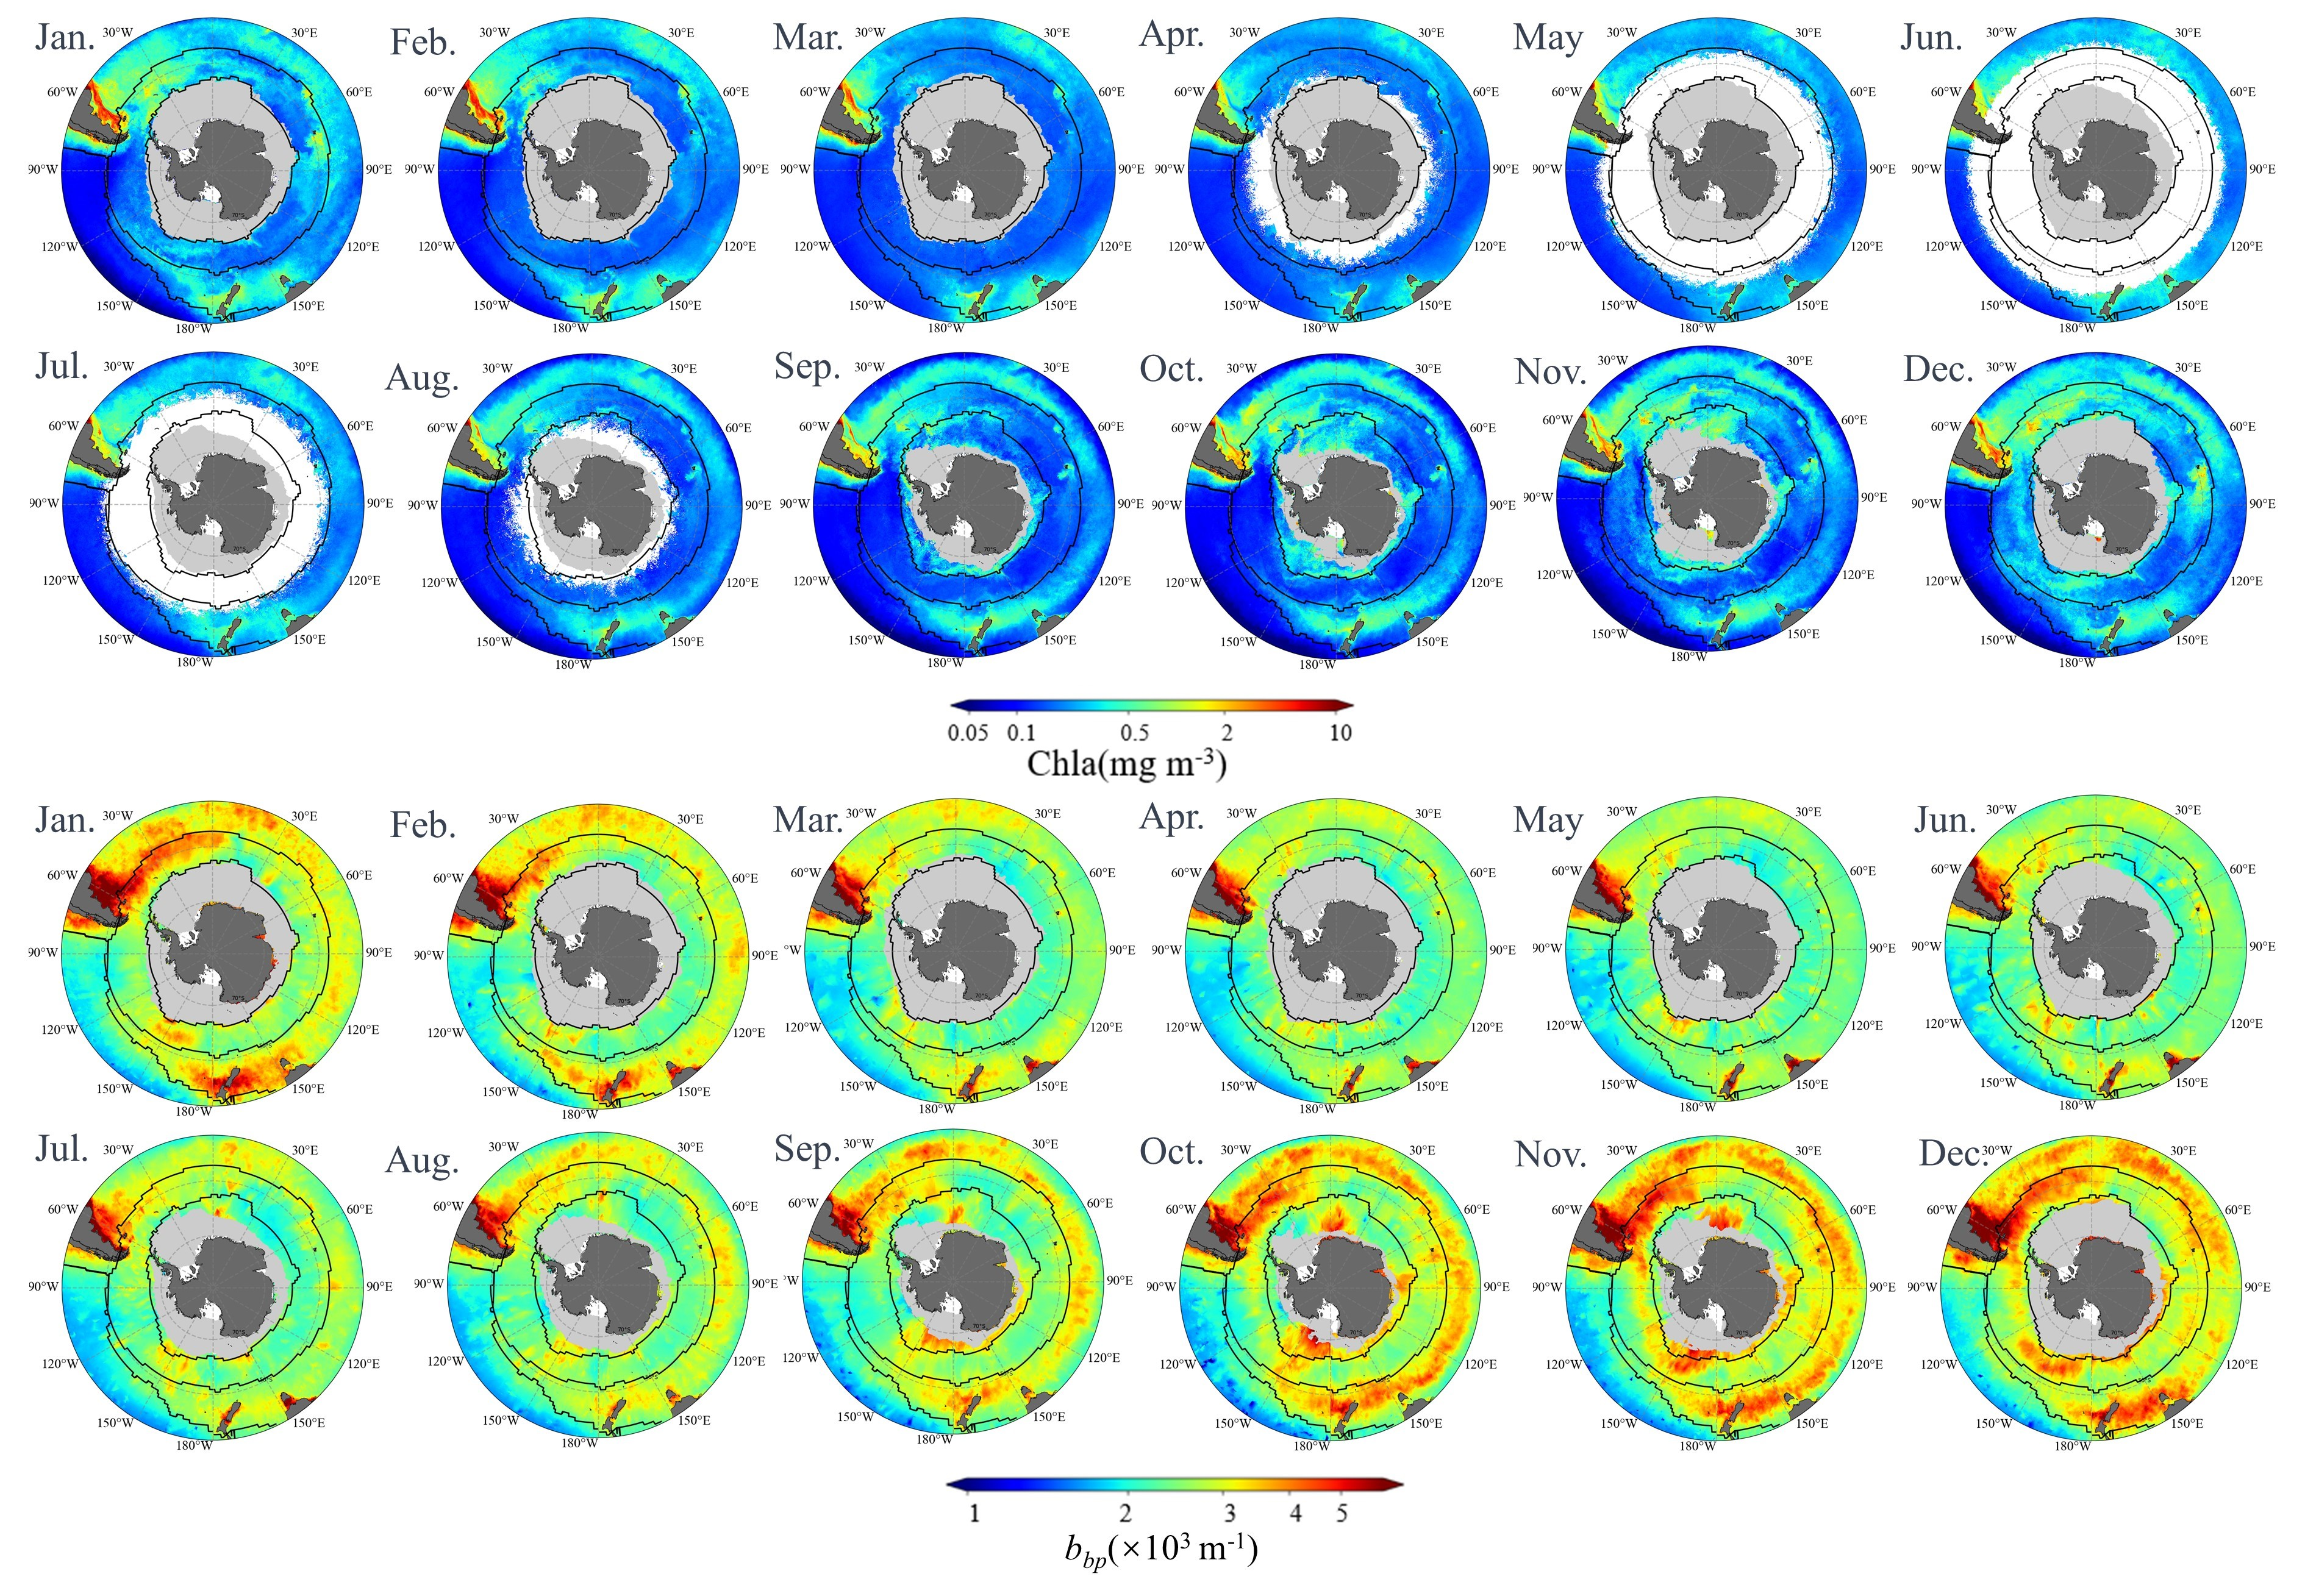
\includegraphics[width=\linewidth]{figure/第三章用图/图3.1.jpg}   
    \bicaption{\label{fig:bbp和叶绿素}Chl-a和插值后的$b_{bp}$月平均分布}{Monthly average distribution map of Chl-a and $b_{bp}$}
\end{figure}
%考虑到$b_{bp}$的成像特点,我们将其进行二维线性插值到0.25°×0.25°空间分辨率,结合其数据产品的数量与质量,我们使用了每月的白天、夜间的数据,根据经纬度信息映射到网格中,网格个若有多个值则计算平均值,在这些平均值的基础进行二维线性插值,这样最终得到了2008年1月~2016年12月的月平均$b_{bp}$数据。

如\autoref{fig:bbp和叶绿素}是Chl-a和插值后的$b_{bp}$数据(插值过程参考第2.2小节)在研究区间内月平均分布图,这些数据为我们的研究提供了基础和依据。从图中可以清楚地看出,作为能够表征生物过程的两种变量$b_{bp}$和Chl-a,两者在空间分布特征上相近,高值基本都是分布在春季的亚热带季节性分层生物群系区域(STSS),这可能与这个季节生物活动的增加有关。Behrenfeld等人\cite{2013Space}发现基于$b_{bp}$得出的浮游植物生物量与海洋生物生态具有一致性的位置分布和季节变化,其在极地地区的研究也证明了这一点\cite{bbp_Annual_2017}。而我们的插值结果进一步印证了Berenfled等人\cite{2013Space,bbp_Annual_2017}的研究结果的正确性,表明$b_{bp}$完全可以用于表征生物泵的作用。

相较而言,MODIS卫星在冬季的观测能力有限,Chl-a的冬季高纬度数据在观测结果中明显缺失(5,6,7月),而基于CLIPSO卫星的$b_{bp}$数据能够实现冬季高纬度数据的测量(82°N$\sim$82°S),我们使用插值结果填补上该区域,从而实现缺失数据的补充,提供更全面的数据支持,使我们能够更准确地理解和分析南大洋$p\mathrm{CO_2}$连续季节的变化。

\subsection{训练数据集的构建}
\begin{table}[htbp]
\centering
\bicaption{\label{tab:数据集}数据集中包含的变量信息}{The variable information contained in the data set}
\begin{tabularx}{\textwidth}{>{\centering\arraybackslash}p{1.5cm}>{\centering\arraybackslash}p{2.5cm} *{3}{>{\centering\arraybackslash}X}}
\toprule
变量   & 数据源     & 时间分辨率 & 空间分辨率       & 处理方式 \\ \midrule
$p\mathrm{CO_2}$ & SOCAT   & /     & /           & /    \\
$b_{bp}$  & CALISOP & 每月    & 0.25°×0.25° & 线性插值 \\
SST  & Aqua    & 月平均   & 4km         & 重采样  \\
MLD  & HYCOM   & 月平均   & 9km         & 重采样  \\
SSS  & EUO     & 月平均   & 9km         & 重采样  \\
wind & CCMP    & 月平均   & 0.25°×0.25° & /    \\
xCO2 & MBL     & 1天    & /           & /    \\ \bottomrule
\end{tabularx}
\end{table}

根据\autoref{equ:pCO2}将SOCAT V2023数据集中的$f\mathrm{CO_2}$修正后得到$p\mathrm{CO_2}$的观测样本后,将观测数据集网格化到0.25°×0.25°的网格中。为了减小误差,将每个航次分开进行处理,由于同一航次内$p\mathrm{CO_2}$采样点相对来说比较接近,显著小于卫星遥感及再分析数据的0.25°×0.25°空间分辨率(约25km×25km),因此,如果在相同的网格中有多条记录,则选择网格中的中值作为有效数据,以确保一组变量数据对应唯一$p\mathrm{CO_2}$值。最后得到约9万条数据,$p\mathrm{CO_2}$数据范围从56μatm到550μatm。

由于遥感数据和再分析数据以及插值结果在空间分辨率上存在差异,我们将所有的数据产品空间分辨率统一到0.25°×0.25°。这里使用了基于Python的CV库中的resize函数实现重采样。根据观测数据集中每条数据的位置和时间信息匹配对应的环境变量值(包括:月平均$b_{bp}$,月平均SST,月平均MLD,月平均SSS,月平均wind,月平均$x\mathrm{CO_2}$),如\autoref{tab:数据集}总结了各个环境变量的来源和处理过程。考虑到遥感数据受到云雾等噪声的影响,我们在匹配环境变量时,使用了3×3的网格均值用作最后匹配值。模型要求保证输入变量非空,排除某些环境变量未匹配到的数据记录后,最终得到包含88890条数据的训练数据集合。

\section{模型建立与结果分析}
\subsection{建模过程与算法评估指标}
\subsubsection{算法评估指标}
在回归类型的机器学习过程中,通常需要评估指标来评估预测值和真实值之间的拟合关系,从而量化模型的性能。在本研究中选择了比较常见的决定系数(Coefficient of Determination, $\mathrm{R^2}$)、均方根误差(Root Mean Squared Error, RMSE)、平均绝对误差(Mean Absolute Error, MAE)来量化。

$\mathrm{R^2}$,也称为拟合优度(Goodness of Fit),能够表示模型预测值与真实值之间的相关程度,它衡量了模型对数据拟合的好坏。对于实际测量值{$y_1,y_2,y_3...y_n$}和预测估计值{$x_1,x_2,x_3...x_n$},相关系数$\mathrm{R^2}$为:
\begin{equation}
    \label{equ:R2}
\mathrm{R^2}=\frac{\sum\limits_{i=1}\limits^{n}\left(\widehat{y_i}-\bar{y_i}\right)^2}{\sum\limits_{i=1}\limits^{n}\left(y_i-\bar{y_i}\right)^2}=1-\frac{\sum\limits_{i=1}\limits^{n}\left(y_i-\widehat{y_i}\right)^2}{\sum\limits_{i=1}\limits^{n}\left(y_i-\bar{y_i}\right)^2}
\end{equation}
% \begin{equation}
%     \label{equ:sample}
%     A=\overbrace{(a+b+c)+\underbrace{i(d+e+f)}_{\text{虚数}}}^{\text{复数}}
% \end{equation}

\autoref{equ:R2}中,$\bar{y_i}$表示测量值平均值,$\widehat{y_i}$表示$x_i y_i$的回归方程,即 $\widehat{y_i}=\widehat{a}+\widehat{b} x_i$ ,且由最小二乘法得:
\begin{equation}
    \label{equ:R2-b}
\widehat{b}=\frac{\sum \limits_{i=1}\limits^{n} x_iy_i-n\bar{x_i}\bar{y_i}}{\sum \limits_{i=1}\limits^{n}x_i^2-n\bar{p_i}}
\end{equation}
\begin{equation}
    \label{equ:R2-a}
    \widehat{a}=\bar{y}_i-\widehat{b}\bar{p_i}
\end{equation}

$\mathrm{R^2}$的值越接近1,说明模型的预测效果越好;如果$\mathrm{R^2}$为负值,则表示模型比随机猜测还差。RMSE,也称为标准误差,其计算公式为:
\begin{equation}
    \label{equ:RMSE}
    RMSE=\sqrt{\frac{\sum\limits_{i=1}\limits^{n}\left(y_i-p_i\right)^2}{n}}
\end{equation}
RMSE对预测值中的大误差(离群点)非常敏感,因为误差在平方后会被放大。因此,RMSE能够很好地反映模型对极端值的处理能力。
MAE表示预测值和观测值之间绝对误差的平均值,衡量了模型预测值与真实值之间的平均偏差。与RMSE相比,MAE对离群点的敏感性较低,因为它没有将误差平方。因此,当数据中存在离群点时,MAE可能是一个更稳健的评估指标。
\begin{equation}
    \label{equ:MAE}
    MAE = \frac{1}{n}\sum\limits_{i=1}\limits^{n}|x_i-y_i|
\end{equation}

\subsubsection{XGBoost算法介绍}
极限梯度提升(eXtreme Gradient Boosting, XGBoost)算法在各类数据科学和机器学习竞赛中取得了显著的成绩,包括 Kaggle,KDDCup,和ACM RecSys等\cite{abou2018xgboost,dhaliwal2018effective}。且在多数的$p\mathrm{CO_2}$反演算法研究中,均表明能够实现准确的预测\cite{stamell2020strengths,joshi2022modeling,song2023construction,gloege2022improved},比如L. Gloege等人\cite{gloege2022improved}利用SST、MLD、xCO2等数据,基于XGBoost算法构造出全球1982-2018年的全球碳汇产品,结果显示对比其他产品,其能够更好地贴合独立观测数据。本研究主要也应用了XGBoost算法用于建立反演模型,这里对其原理及其优点进行介绍。

XGBoost算法是在2016年\cite{2016XGBoost}由Chen和Guestrin基于梯度提升决策树(Gradient Boosting Decision Tree, GBDT)算法提出的改进的Boosting算法。GBDT算法采用梯度下降的思想不断迭代模型,每一次迭代需要生成一颗新的树,以生成的所有的树为基础,朝着最小给定目标函数方向前进。XGBoost算法利用了CPU的多线程特点进行并行计算,同时运用集成学习的方法将多个弱学习器集成到一个强学习器,在目标函数上引入泰勒公式来近似和拟合目标函数,在过程中加入正则化目标项来控制模型的复杂度来防止过拟合。其模型原理如下:对于给定的包含有m个特征的n条数据的样本集${x_1,x_2,…,x_n}(x=n),x_i\in R^m$ ;XGBoost算法利用m个特征生成多个树基模型,且每一个基模型利用上一个基模型的残差以提高决策效果,通过下式进行预测:

\begin{equation}
    \label{equ:xgb-1}
   \widehat{y_i}= \sum _{i=1}^{N}f_k(x_i),f_k\in F
\end{equation}
式中,$y_i$是模型的预测值,N是树模型的数量,$f_k$表示第k个树模型,F表示所有的回归树。在XGBoost算法的每一次迭代过程中,都会将一个新的函数添加到模型中,一个的函数对应一棵树,新生成的树则会拟合上次预测的残差,迭代过程如下:

\begin{equation}
    \label{equ:xgb-2}
    \left\{
        \begin{aligned}
        \widehat{y_i}^{(0)} &= 0\\
        f_1(x_i) &= \widehat{y_i}^{(1)} = \widehat{y_i}^{(0)} + f_1(x_i) \\
        \widehat{y_i}^{(t)} &= \widehat{y_i}^{(t-1)} + f_t(x_i)
        \end{aligned}
    \right.
\end{equation}

XGBoost算法为了预测更加精准并且增大泛化能力,在目标函数中增加了损失函数和正则项,其中损失函数用来调整训练函数,正则项用来简化模型,以防止过拟合。如下式:

\begin{equation}
    \label{equ:xgb-3}
   L(O)=\sum_{i=1}^nL(y_i,\widehat{y_i}^{(t-1)}+f_t(x_i))+\sum_k \Omega(f_k)
\end{equation}

其中,$y_i$是真实值,L(0)是目标函数,第二项是损失函数,其中,$\widehat{y_i}^{(t-1)}$表示保留前面t-1轮的模型预测,$f_t(x_i)$表示一个新的函数。最后一项是正则项。XGBoost算法将损失函数通过Taylor公式展开来逼近真实值,如下式:
\begin{equation}
    \label{equ:xgb-4}
   L(y_i,\widehat{y_i}^{(t-1)} +f_t(x_i)) = L(y_i,\widehat{y_i}^{(t-1)})+g_if_i(x_i)+\frac{1}{2}h_if_t^2(x_i)
\end{equation}

于是目标函数近似为下式:
\begin{equation}
    \label{equ:xgb-5}
   L\left(O\right)=\sum_{i=1}^{n}\left[L\left(y_i,\widehat{{y_i}^{\left(t-1\right)}}\right)+g_if_i\left(x_i\right)+\frac{1}{2}h_if_t^2\left(x_i\right)\right]+\sum_{k}{\Omega\left(f_k\right)\ }
\end{equation}

\subsubsection{模型训练过程}
在机器学习中,为了得到一个性能优秀的模型,数据集通常被分为了三个部分,即训练集、验证集和独立测试集。分析数据我们发现,在同一个航次内$p\mathrm{CO_2}$数值较为相近且连续;如果直接从整体的数据集中随机抽取作为独立测试集合,则这部分数据可能会被模型“记住”。为了更好地测试模型的外推能力和泛化能力,我们从全部的航次中随机抽取出了50条航次的实测数据,约6623条数据记录作为独立测试集用,确保这些航次的数据没被被模型学习到。剩下的部分则先通过网格算法来进行超参数寻优,参数确定之后,我们继续进一步验证模型的准确性和稳定性,即将数据集分成两部分,其中70\%用于训练,30\%用于验证,过程中使用了三次交叉验证来测试模型的准确性和稳定性。

\subsubsection{网格搜索算法优化}
为了发挥出XGBoost算法的最好效果,需要调整一系列的参数,其中主要有通用参数、辅助参数以及任务参数。通用参数用来确定算法中选择的上升模型类别,比如booster参数,可设置为gbtree(树形模型)或者gblinear(线性模型),nthread用于设置线程数,默认为最大可用线程数;辅助参数则取决于所选用的上升模型,比如上升模型确定为树形模型时,可通过设置max\_depth设置每棵树的最大深度,值越大,越容易过拟合,设置subsample值可设定 每棵树训练时使用的样本比例,样本权重(subsample)控制每棵树训练时使用的样本比例,较小的样本权重可以提高模型的泛化能力,eta学习率决定每次迭代中新树的权重,较小的学习率可以使模型更加稳定,但可能需要更多的迭代次数;任务参数定义学习任务和相应的学习目标,objective: 定义学习任务和相应的学习目标,eval\_metric: 评估指标,用于验证模型的性能。参数的具体指标可以参考\url{https://xgboost.readthedocs.io/en/stable/parameter.html}。

\begin{table}[htbp]
\centering
\bicaption{\label{tab:网格优化算法}网格优化算法中的参数、步长和最优参数}{Parameters and optimal parameters set by the grid search algorithm}
\begin{tabularx}{\textwidth}{>{\centering\arraybackslash}p{5cm}>{\centering\arraybackslash}p{4cm}>{\centering\arraybackslash}X}
\toprule
超参数    & 范围                &最优值 \\
\midrule
n\_estimators      & 500-2000(步长 =100)  & 1700            \\
learning\_rate     & 0.01-0.2(步长 =0.01) & 0.02            \\
max\_depth         & 5-15(步长 =1)      & 9          \\
gamma              & 0-1.0(步长 =0.1)     & 0.05            \\
subsample          & 0.7-1.0(步长 =0.1)   & 0.8             \\
alpha              & 0-0.1 (步长 =0.01)    & 0.05            \\
min\_child\_weight & 1-10(步长 =1)      & 6               \\
colsample\_bytree  & 0.5-1.0(步长 =0.1)        & 0.8             \\
\bottomrule
\end{tabularx}
\end{table}
为了提高模型训练的效率和精度,我们使用网格搜索进行优化,并以决定系数$\mathrm{R^2}$作为评价标准。网格搜索算法可以被自动化地应用到机器学习流水线中,使得模型训练的过程更加高效、自动化。另外,我们在过程中设置了K折交叉验证(K=5),能够将数据集划分为训练集和验证集的5个不同子集,并且多次训练模型,每次使用不同的子集作为验证集,从而得到模型性能的稳健估计。过程中设置的各参数范围、寻优步长和最优参数详见\autoref{tab:网格优化算法}。

%---------------------------------------------------------------
%---------------------------------------------------------------
%---------------------------------------------------------------
%---------------------------------------------------------------

\subsection{模型表现及不同算法间的比较}
\subsubsection{基于XGBoost算法模型表现}

\begin{table}[htbp]
\centering
\bicaption{\label{tab:三次交叉验证结果}三次交叉验证结果}{Results of three cross-validations}
\begin{tabularx}{\textwidth}{>{\centering\arraybackslash}p{1.5cm}>{\centering\arraybackslash}p{1.5cm} *{3}{>{\centering\arraybackslash}X}}
\toprule
集合 & 序号 & RMSE($\mu atm$) & MAE($\mu atm$) & $\mathrm{R^2}$ \\ \midrule
     & 1    & 2.15            & 1.45           & 0.99  \\
训练  & 2    & 2.89            & 1.79           &0.99       \\
     & 3    & 2.34            & 1.64           & 0.99      \\
     & 平均 &  2.46±0.31       &  1.62±0.13     & 0.99±0.00  \\ \midrule
     & 1    & 13.47           & 8.21           & 0.82  \\
验证  & 2   &  14.51           &  9.10          &  0.83     \\
     & 3    &  14.67          &  8.56          &  0.82     \\
     & 平均 &  13.88±0.60      & 8.62±0.43     &   0.82±0.0058 \\ \bottomrule
\end{tabularx}
\end{table}
\autoref{tab:三次交叉验证结果}展示了网格搜索算法寻优后得到的XGBoost算法模型三次交叉验证结果,过程中已经确保了每次使用的训练集和验证集不相同。模型的结果表明,该算法能够非常精确地进行预测和拟合。三次交叉验证的训练集合中,RMSE为2.46±0.31 μatm,MAE为1.62±0.13,$\mathrm{R^2}$为0.99±0.00;在验证集的表现中,RMSE为13.88±0.60 μatm,MAE为8.62±0.43μatm,$\mathrm{R^2}$为0.82±0.0058。三次验证结果中最优成绩如\autoref{fig:fig-3.2}所示,在训练集中,有52861条数据,模型表现良好,RMSE仅为2.15,MAE为1.45,$\mathrm{R^2}$为0.99;在验证集的22655条数据中,模型的RMSE为13.47,MAE为8.21,R2为0.82。且验证集和训练集中的大多数点均处于反演 $p\mathrm{CO_2}$ 和实测 $p\mathrm{CO_2}$ 的 1:1 等位线附近,说明验证集数据对于XGBoost算法所建立的模型仍具有较为优异的结果,通过XGBoost算法在南大洋地区反演 $p\mathrm{CO_2}$ 可以取得准确且可靠的效果。后续的反演使用的模型则是基于最优一次训练结果。

\begin{figure}[htbp]
    \centering
    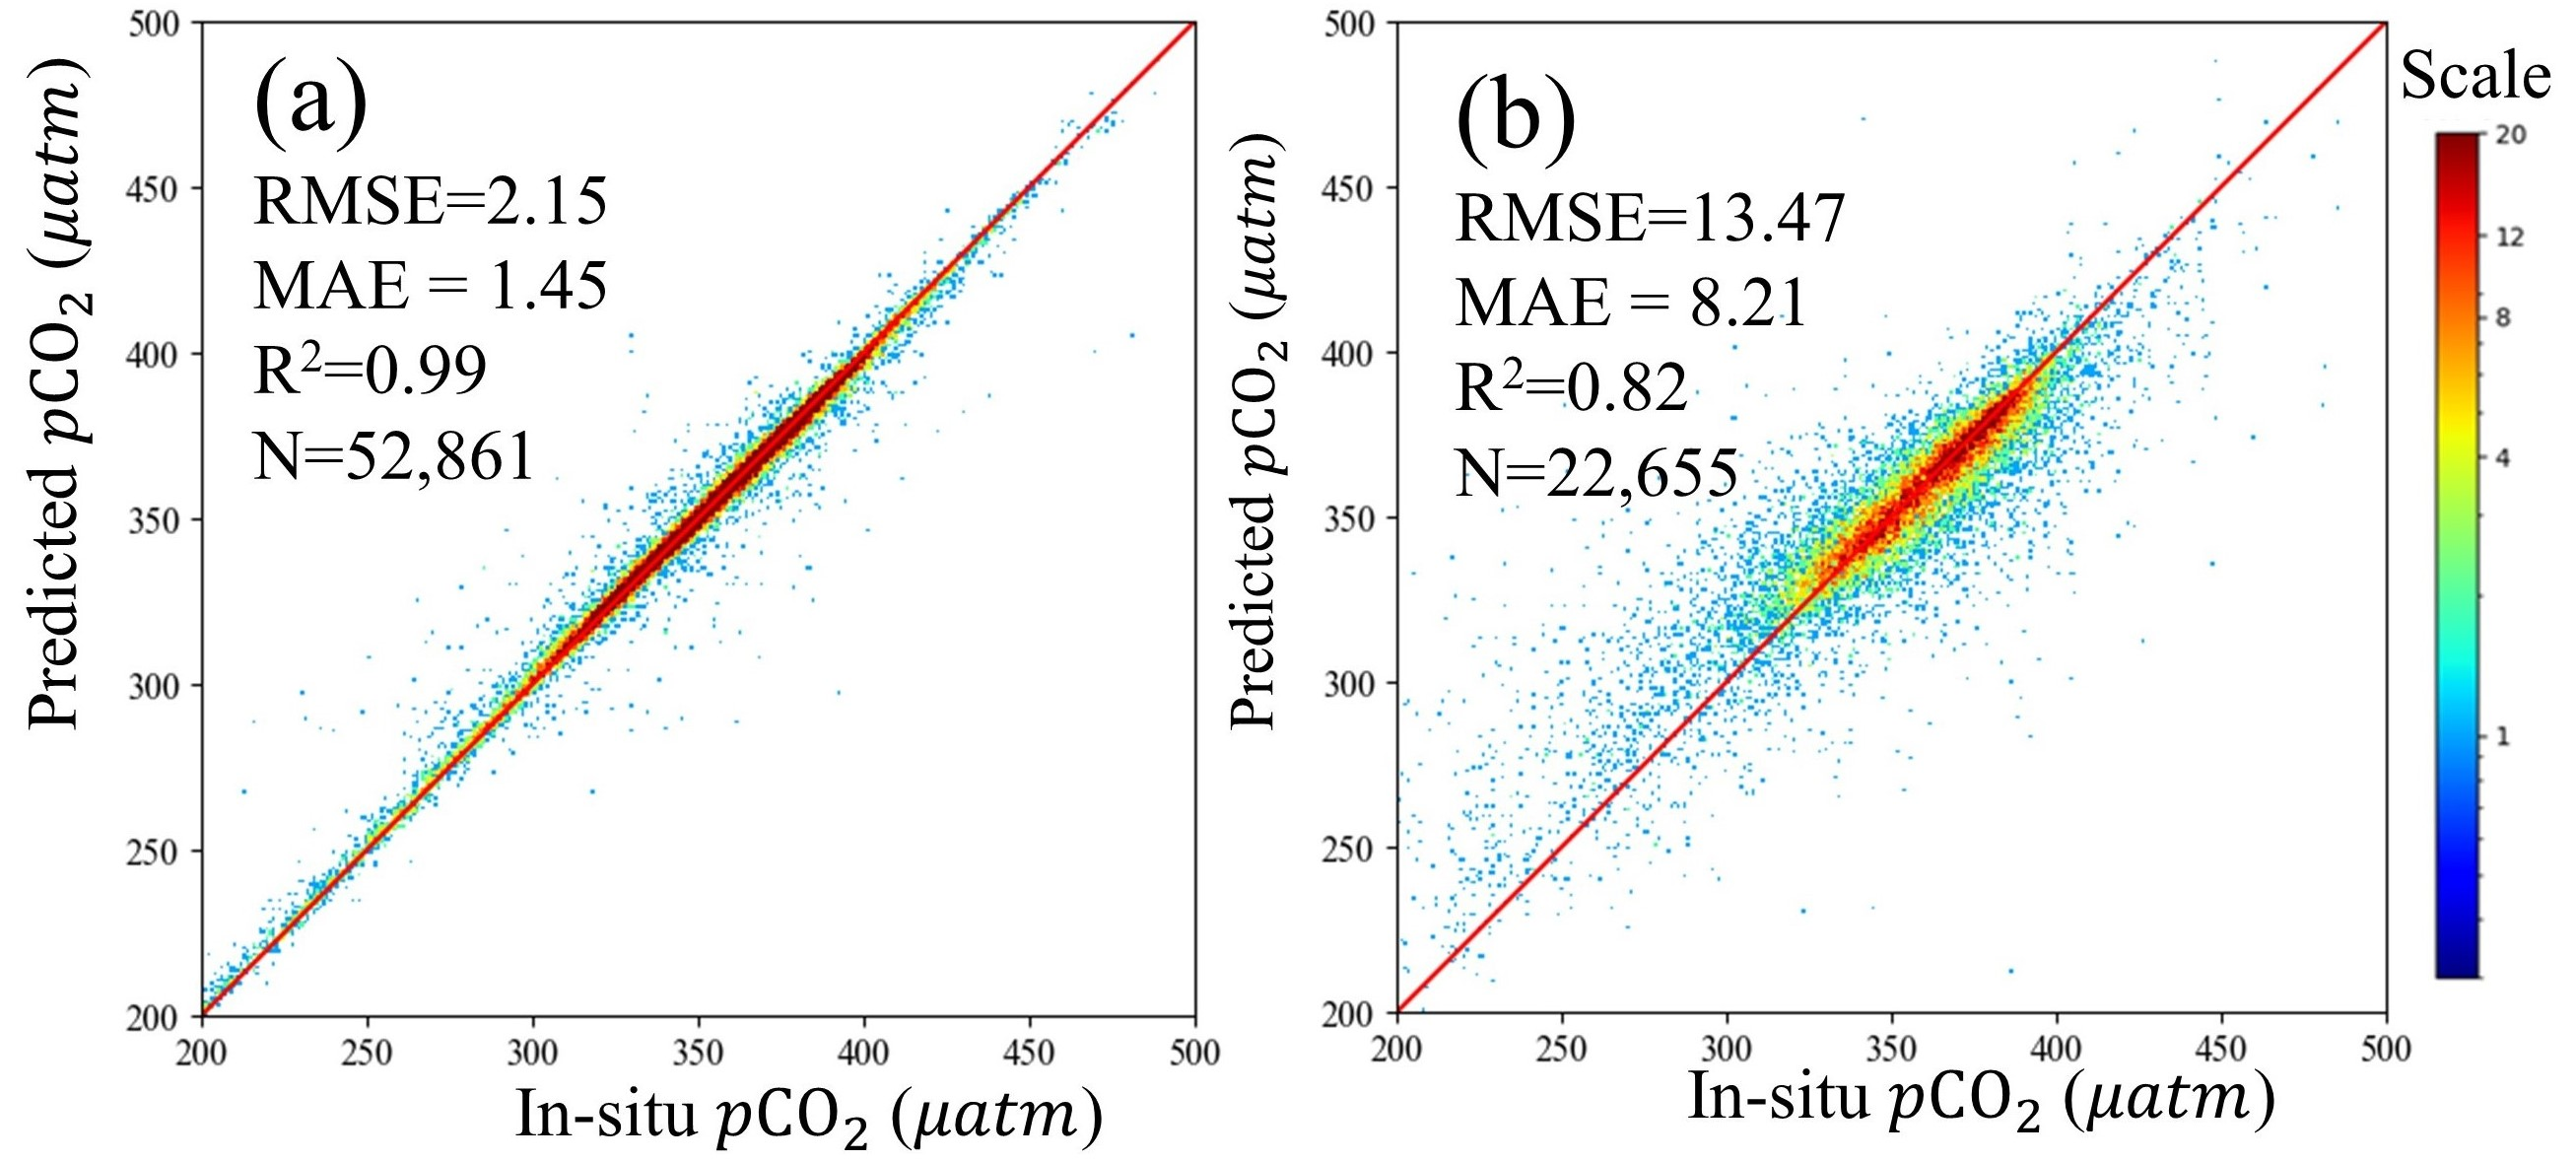
\includegraphics[width=\linewidth]{figure/第三章用图/图3.2.jpg}
    \bicaption{\label{fig:fig-3.2}(a)模型训练集结果和(b)验证集结果}{(a) Model training set results and (b) validation results}
\end{figure}

\subsubsection{不同算法间的表现}
\begin{table}[htbp]
\centering
\bicaption{\label{tab:不同算法}不同算法结果的对比(验证集对比结果)}{Comparison of different algorithm results}
    \begin{tabularx}{\textwidth}{>{\centering\arraybackslash}X m{2cm} m{2cm} m{2cm}}
    \toprule
    算法  & RMSE($\mu atm$) & MAE($\mu atm$) & $\mathrm{R^2}$  \\ \midrule
    线性回归                    &  27.82  &  23.23  & 0.41  \\
    k 邻近算法                  & 27.82 & 27.82 & 0.56 \\
    前向神经网络                 & 19.48 & 20.18 & 0.76 \\
    回归树                      & 20.98 & 19.22  &0.70   \\
    支持向量机-高斯核函数         & 21.11 & 17.37 & 0.67 \\ 
    支持向量机-线性核函数         & 20.59 & 18.39 & 0.68 \\ 
    随机森林                    & 18.53 & 21.68 & 0.70 \\
    Bagging回归                 & 17.02 &18.88  &0.74\\
    自适应增强算法               &19.23  & 18.48 &0.73 \\
    梯度提升树算法               & 17.54 &17.19 & 0.71 \\
    \bottomrule
    \end{tabularx}
\end{table}

本小节旨在探究南大洋海表$p\mathrm{CO_2}$反演过程中不同机器学习算法的应用效果。我们对比了几种常见的回归类型的机器学习算法,包括k邻近算法、支持向量机(SVM)、神经网络,以及集成学习算法(如随机森林、自适应增强算法、梯度提升树算法和Bagging回归)等基本方法。为了确保结果的可比较性,我们采用了一致的方法。具体而言,我们将数据集按照3.1小节的建议进行训练集和验证集的划分。首先,我们对需要调优的几种算法均采用网格搜索算法对模型参数进行优化。然后,通过三次交叉验证来验证模型的准确性和稳定性,最终使用验证集计算RMSE(均方根误差)、MAE(平均绝对误差)和$\mathrm{R^2}$(决定系数)等关键统计指标,评估各算法对该数据集的验证效果。

各个算法三次交叉验证的最优结果如\autoref{tab:不同产品对比}所示,这些算法结果表明,多个学习器组合成的集成学习方法的表现要优于单个学习器;传统的线性回归模型在这里表现很差,RMSE、$\mathrm{R^2}$均为所有算法中最高的,拟合效果较差,难以应用在情况较为复杂的南大洋地区。基于树型学习器的多种算法效果均表现良好,他们的$\mathrm{R^2}$均超过了0.7,且RMSE均均小于20μatm。
另外在上述的集成算法中,Bagging回归和梯度提升算法均取得了不错的效果,效果略低于XGBoost算法。结合所有算法的结果,XGBoost算法的效果最为突出,三个指标均比其他算法好,具有较高的准确度,因此本研究最终采用XGBoost算法反演南大洋海表$p\mathrm{CO_2}$。

\subsection{模型独立验证结果与敏感度分析}
\subsubsection{模型独立验证结果}
\begin{figure}[htbp]
    \centering
    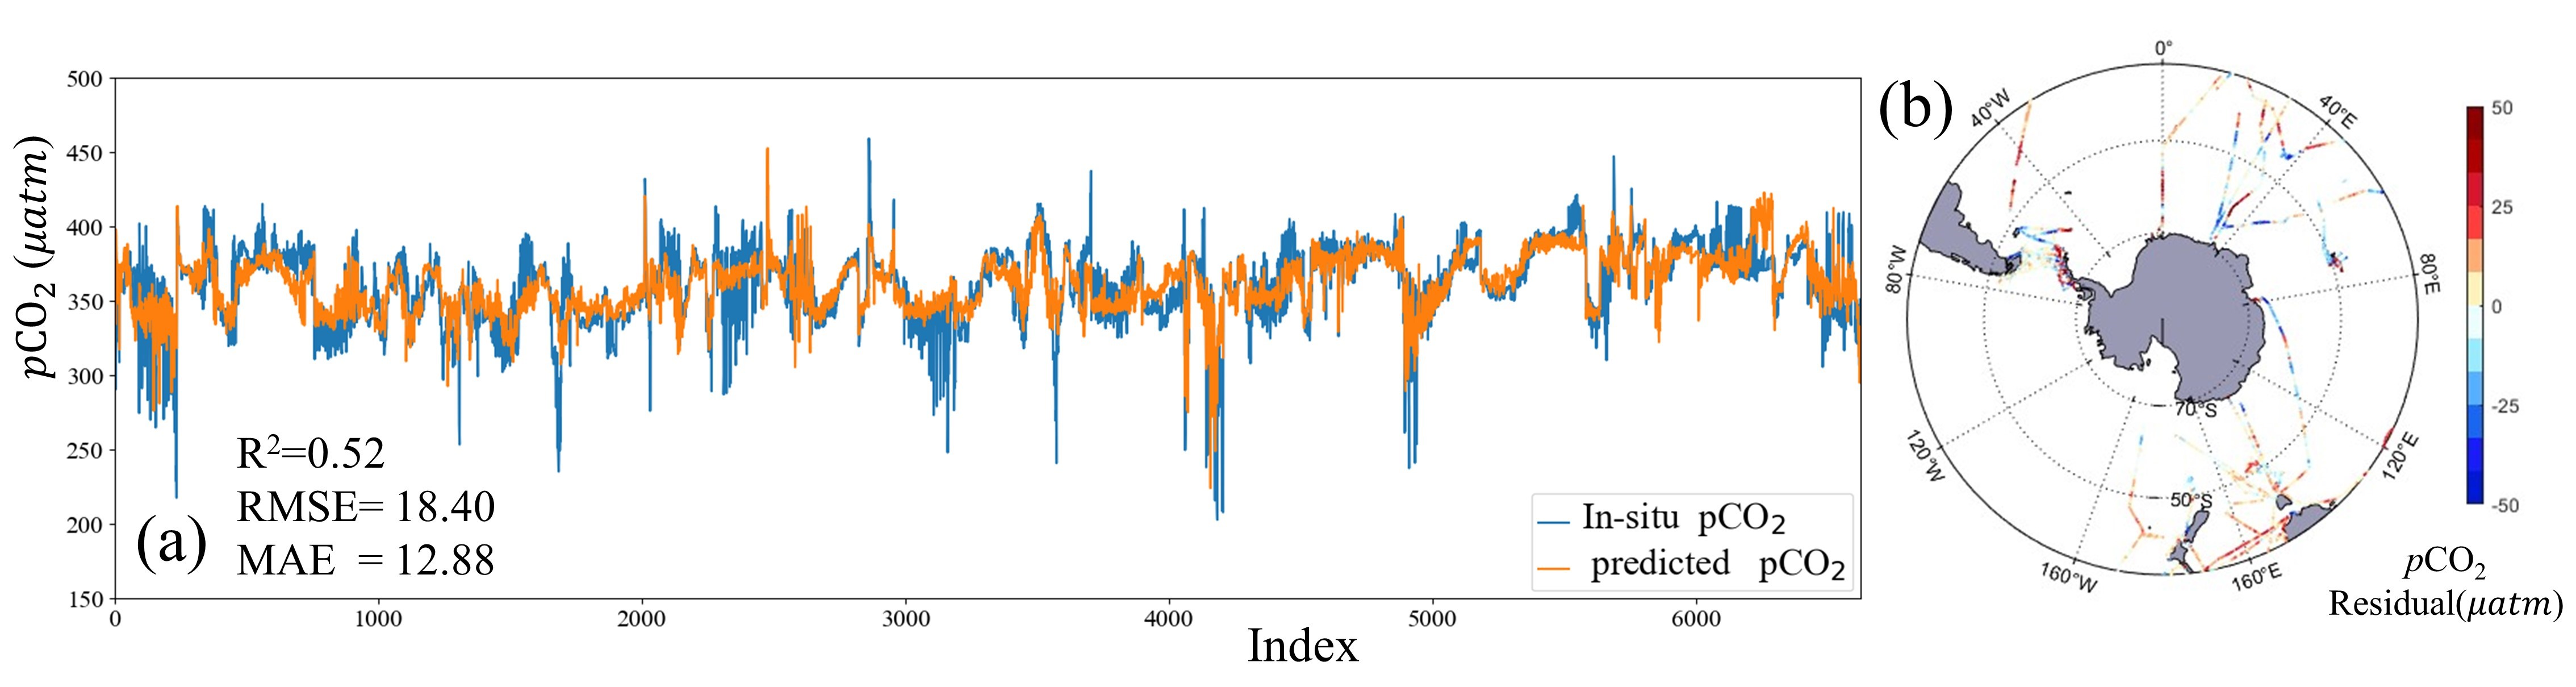
\includegraphics[width=\linewidth]{figure/第三章用图/图3.3.jpg}
    \bicaption{\label{fig:独立验证}
    (a) 随机抽取的50条走航数据的现场海面$p\mathrm{CO_2}$与XGBoost模型预测的海表$p\mathrm{CO_2}$的比较;(b) 随机抽取的50条走航数据的分布以及残差(观测值-预测值)情况}
    {(a) the comparison between in-situ sea surface $p\mathrm{CO_2}$ and sea surface $p\mathrm{CO_2}$ predicted by the XGB-model for the 50 randomly selected cruises; (b) distribution of randomly selected 50 cruises and their residuals.}
\end{figure}

在训练过程中我们预留了五十条走航数据没有参与训练过程,用作独立测试集,此举可用于验证模型的外推能力。这50条随机抽选的航次分布情况如\autoref{fig:独立验证}-(b)所示,基本覆盖了南大洋的各个区域。 \autoref{fig:独立验证}-(a)中我们能看到模型能够很好地拟合,且能够抓住变化趋势。从数据角度来看,RMSE为18.40μatm,MAE为12.88μatm,$\rm R^2$为0.52,说明模型you较好的拟合效果。\autoref{fig:独立验证}-(b)为残差图,可以看到除去东经160°,南纬35°的近岸地区误差较大外,模型误差较小,说明该模型完全有把握地预测南大洋$p\mathrm{CO_2}$时空变化。

\subsubsection{敏感性验证}
\begin{table}[htbp]
\centering
\bicaption{\label{tab:敏感性统计}模型对每个输入变量不确定性的敏感性统计}{Model sensitivity statistics to uncertainty in each input variable}
\begin{tabularx}{\textwidth}{>{\centering\arraybackslash}p{2cm} >{\centering\arraybackslash}p{3cm} >{\centering\arraybackslash}p{3cm} >{\centering\arraybackslash}p{1.5cm} >{\centering\arraybackslash}p{1.5cm} >{\centering\arraybackslash}p{1.5cm}}
\toprule
变量                       & 输入范围                            & 调整    & RMSE & MAE & $\rm R^2$ \\ \midrule
\multirow{2}{*}{$b_{bp}$} & \multirow{2}{*}{-0.0031$\sim$0.023} & +20\% & 14.16   & 8.59  & 0.80        \\
                          &                                     & -20\% & 14.13   & 8.57  & 0.80      \\
\multirow{2}{*}{SST}      & \multirow{2}{*}{-1.80$\sim$25.10}   & +1°C & 14.13   & 8.56  & 0.80        \\
                          &                                     & -1°C & 14.12   & 8.57  & 0.80         \\
\multirow{2}{*}{MLD}      & \multirow{2}{*}{8.75$\sim$400.00}   & +20\% & 14.13   & 8.57  & 0.80        \\
                          &                                     & -20\% & 14.13   & 8.57  & 0.80       \\
\multirow{2}{*}{SSS}      & \multirow{2}{*}{3.87$\sim$36.97}    & +20\% & 14.13   & 8.58 & 0.80         \\
                          &                                     & -20\% & 14.13   & 8.58 & 0.80       \\
\multirow{2}{*}{wind}     & \multirow{2}{*}{2.42$\sim$15.28}    & +20\% & 14.13  & 8.58  & 0.80       \\
                          &                                     & -20\% & 14.13   & 8.58 & 0.80       \\
\multirow{2}{*}{$x\mathrm{CO_2}$} & \multirow{2}{*}{381.75$\sim$402.02} & +0.0073ppm & 14.13    & 8.57 & 0.80        \\
                          &                                     & -0.0073ppm & 14.13   & 8.57  & 0.80        \\ \bottomrule
\end{tabularx} 
\end{table}

在进行模型分析的过程中,我们必须认识到每个输入变量都存在一定的测量不确定性。这种不确定性无疑会对$p\mathrm{CO_2}$的反演结果产生影响。为了更深入地理解这种影响以及模型对输入变量不确定性的敏感度,本小节将采取一种实验性的方法,即通过在输入变量中添加噪声来更好地理解模型对输入变量不确定性的反应,从而改进我们的模型,也有助于我们评估模型的稳健性,并为进一步的模型改进提供依据。
\begin{figure}[htbp]
    \centering
    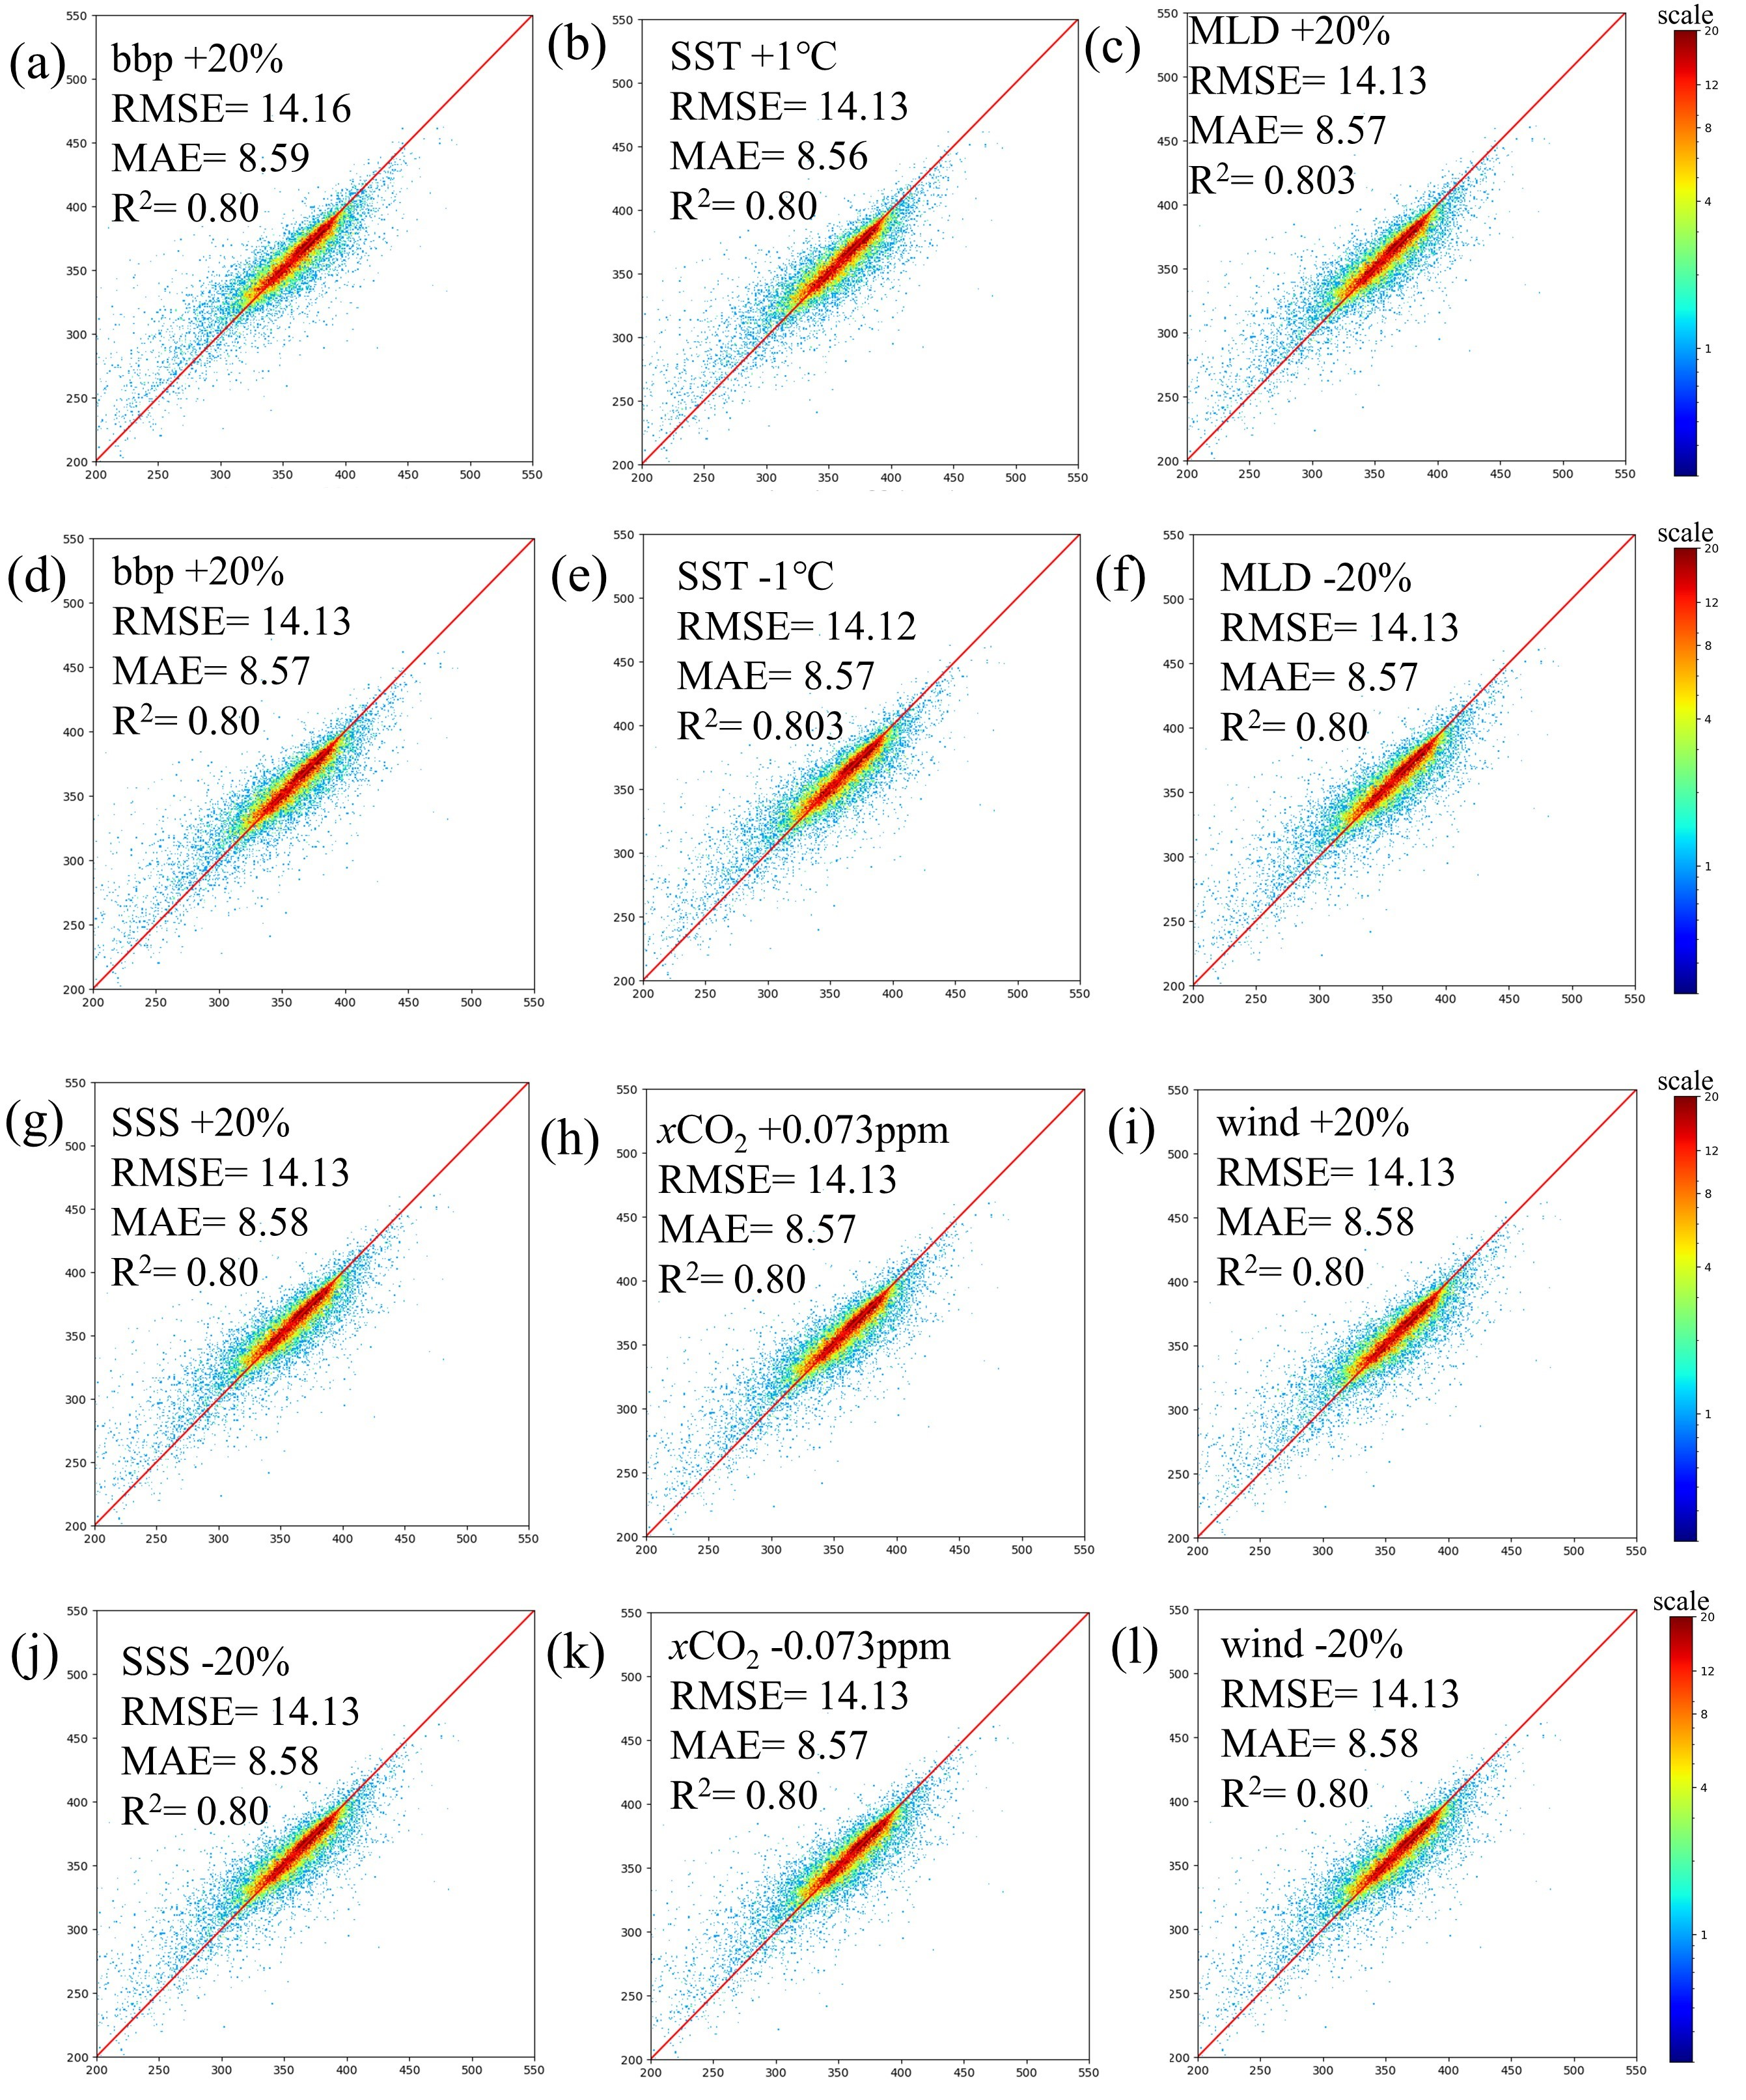
\includegraphics[width=\linewidth]{figure/第三章用图/图3-敏感度分析.jpg}
    \bicaption{\label{fig:fig-敏感度分析}各个变量敏感度分析验证集结果,横轴为实测$p\mathrm{CO_2}$,纵轴为预测$p\mathrm{CO_2}$}{Sensitivity analysis of various variables, validation set results. The X-axis represents observed $p\mathrm{CO_2}$, while the Y-axis represents predicted $p\mathrm{CO_2}$. }
\end{figure}

相关研究表明,来自MODIS卫星的SST数据通常存在着±1°C的不确定性\cite{hu2009building},对于$x\mathrm{CO_2}$数据其观测站点的不确定度约在±0.073ppm\cite{dlugokencky2021atmospheric},而其他的数据产品通常取±20\%的不确定性。通过对变量添加不确定度噪声之后,结果如\autoref{fig:fig-敏感度分析}所示,总的来说,模型对于噪声的输入变化很小,说明了模型足够稳健。其中,模型对以$b_{bp}$为代表的生物泵作用最为敏感,而对于其他输入环境变量而言,模型则不敏感。

%===================================================================================
%===================================================================================
%===================================================================================
%===================================================================================
%===================================================================================

\section{本章小结}

本章节主要讲述了基于机器学习算法建立$p\mathrm{CO_2}$反演模型的过程,包括建模步骤及模型性能表现情况。本章节包含两个主要部分:一是训练前数据集的构建,二是模型的建立和验证。

在第一部分,首先介绍了本研究中使用的$b_{bp}$插值结果,作为能够表征浮游植物生物量变化的变量,其地理、时间分布情况与Chl-a类似,同时可以补充冬季数据。因此,我们将其加入模型中,确保模型能学习到生物过程对$p\mathrm{CO_2}$的影响。此外,我们还介绍了训练过程中构建的数据集,包含$p\mathrm{CO_2}$、$b_{bp}$、SST、SSS、wind、$x\mathrm{CO_2}$、MLD等变量,各个变量的空间分辨率都统一到了0.25°×0.25°。除去未匹配到环境变量数据的记录后,总共得到了82,139条有效数据。

在第二部分,我们首先详细介绍了如何建立模型,包括在机器学习回归问题中常用的评估指标和XGBoost算法的详细原理。接着,我们详述了训练过程,包括我们如何通过航次划分数据进行独立测试,以及剩余部分数据如何通过网格搜索算法进行优化。我们使用了70\%的数据进行模型训练,30\%用于验证,同时进行了三次交叉验证,以监测模型的准确性和稳定性。在XGBoost算法训练过程中,我们使用了网格搜索算法进行参数优化,并详细介绍了这个过程。在第二部分的第二小节中,我们对XGBoost模型的训练结果进行了详述,同时也比较了多种常见的机器学习方法。结果表明,XGBoost算法在本研究中的性能最优,最适合用于南大洋$p\mathrm{CO_2}$的反演。在第三小节中,我们对模型的外推能力以及泛化能力进行了分析,使用了独立验证数据集和敏感性分析方法进行验证。结果表明,该模型具有实现$p\mathrm{CO_2}$反演的能力,且模型稳定性良好,能够应对输入变量异常的情况。

综上,我们建立了一个能够准确且可靠地用于南大洋$p\mathrm{CO_2}$反演的模型。





























